\chapter{Behavioral clustering}
\section{Experimental design}

\subsection{Conceptual basis}
\subsection{Overview of process}

\section{Similarity matrix creation}

\subsection{Implementation details}
\subsection{Results}

\section{Markov clustering}
\subsection{Background}
\subsection{Tuning parameters}
\subsection{Results}

\section{Categorization of clusters}
\subsection{Implementation details}
\subsection{Results}

\section{Discussion of cluster categories}
\subsection{Implications}
\subsection{Opportunities for future work}
\subsection{Threats to validity}

An ideal analysis of regex behavioral similarity would use subsumption or containment analysis. However, we struggled to find a tool that could facilitate such an analysis. Further, regular expressions in code libraries (e.g., for Python, Java) are not the same as regular languages in formal language theory. Some features of regular expression libraries, such as backreferences, make the libraries more expressive than regular languages. This allows a regular expression pattern to match, for example, repeat words, such as ``cabcab", using the pattern {\tt ([a-z]+)\verb!\!1}. However, building an automaton to recognize such a pattern and to facilitate containment analysis, is infeasible.
For these reasons, we developed a similarity analysis based on string matching.

\begin{figure}[tb]
\centering
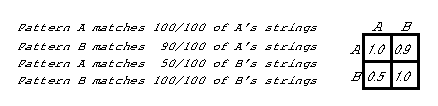
\includegraphics[height=0.6in]{nontex/illustrations/minimalMatrix.eps}
\caption{A similarity matrix created by counting strings matched}
\label{fig:minimalMatrix}
\end{figure}

\begin{figure}[tb]
\centering
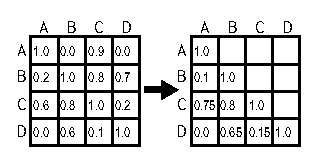
\includegraphics[width=0.7\columnwidth]{nontex/illustrations/matrixToGraph.eps}
\vspace{-6pt}
\caption{Creating a similarity graph from a similarity matrix}
\vspace{-6pt}
\label{fig:matrixToGraph}
\end{figure}

Our similarity analysis clusters regular expressions by their behavioral similarity on matched strings.
Consider two unspecified patterns {\tt A} and {\tt B}, a set {\tt mA} of 100 strings that pattern {\tt A} matches, and a set {\tt mB} of 100 strings that pattern {\tt B} matches.
If pattern {\tt B} matches 90 of the 100 strings in the set {\tt mA}, then {\tt B} is 90\% similar to {\tt A}.
If pattern {\tt A} only matches 50 of the strings in {\tt mB}, then {\tt A} is 50\% similar to {\tt B}.
We use similarity scores to create a similarity matrix as shown in Figure~\ref{fig:minimalMatrix}.
In row {\tt A}, column {\tt B} we see that {\tt B} is 90\% similar to {\tt A}.
In row {\tt B}, column {\tt A}, we see that {\tt A} is 50\% similar to {\tt B}.  Each pattern is always 100\% similar to itself, by definition.

Once the similarity matrix is built, the values of cells reflected across the diagonal of the matrix are averaged to create a half-matrix of undirected similarity edges, as illustrated in Figure~\ref{fig:matrixToGraph}.
This facilitates clustering using the  Markov Clustering (MCL) algorithm\footurl{http://micans.org/mcl/}.
We chose MCL  because it offers a fast and tunable way to cluster items by similarity and it is particularly useful when the number of clusters is not known \emph{a priori}.


In the implementation, strings are generated for each pattern using Rex~\cite{rex}.  Rex generates matching strings by representing the regular expression as an automaton, and then passing that automation to a constraint solver that generates members for it\footurl{http://research.microsoft.com/en-us/projects/rex/}.  If the regex matches a finite set of strings smaller than 400, Rex will produce a list of all possible strings.
Our goal is to generate 400 strings for each pattern to balance the runtime of the similarity analysis with the precision of the similarity calculations.

For clustering, we prune the similarity matrix to retain all similarity values greater than or equal to 0.75, setting the rest to zero, and then using MCL.
This threshold was selected based on recommendations in the MCL manual. The impact of lowering the threshold would likely result  in either the same number of more diverse clusters, or a larger number of clusters, but is unlikely to markedly change the largest clusters or their summaries, which are the focus of our analysis for RQ4
% (Section~\ref{rq4:results})
, but further study is needed to substantiate this claim.
We also note that MCL can also be tuned using many parameters, including inflation and filtering out all but the top-k edges for each node.
After exploring the quality of the clusters using various tuning parameter combinations, the best clusters (by inspection) were found using an inflation value of 1.8 and k=83.   The top 100 clusters are categorized by inspection into six categories of behavior.

The end result is clusters and categories of highly behaviorally similar regular expressions, though we note that this approach has a tendency to over-approximate the similarity of two regexes. We measure similarity based on a finite set of generated strings, but some regexes  match an infinite set (e.g., \verb!ab*c!), so measuring similarity based on the first 400 strings may lead to an artificially high similarity value. To mitigate this threat, we chose a large number of generated strings for each regex, but future work includes exploring other approaches to computing regex similarity.


In clustering the regular expressions, we are most interested in observing behavior of regexes found in multiple projects.  Starting with the 13,597 patterns of the corpus, we discarded 10,015 (74\%) patterns that were not found in multiple projects.
Then we excluded an additional 711 (5\%) patterns that contain features not supported by Rex.  We studied the remaining 2,871 (21\%) patterns using our similarity analysis technique. The impact is that 923 projects were excluded from the data set for the similarity analysis. Omitted features are indicated in Table~\ref{table:featureStats} for Rex.

From 2,871 distinct patterns, MCL clustering identified 186 clusters with 2 or more patterns, and 2,042 clusters of size 1.
 The average size of clusters larger than size one was 4.5.  Each pattern belongs to exactly one cluster.

Three example strings generated by Rex for the first pattern are: `-()', `*'8(5)', `Oe()'.  For the third pattern, Rex generated these three strings: ` ()', `(q)F', `(n)M'.  The pattern: \verb!\(.*\)$! is very similar, but will not match the string `(n)M', and so was placed in a different cluster.

\begin{table}
\begin{center}
\caption{An example cluster containing 12 regexes, with at least one regex present in 31 different projects.  In this cluster, every regex requires `:'.}
\label{table:exampleCluster}
\begin{small}
\begin{tabular}
{lcc | lcc}
\toprule \bigstrut
\textbf{Index} & \textbf{Pattern} & \textbf{NProjects} & \textbf{Index} & \textbf{Pattern} & \textbf{NProjects} \\
 \midrule \bigstrut
1 & \begin{minipage}{1.6in}\cverb!\s*([^: ]*)\s*:(.*)!\end{minipage} & 9 & 7 & \begin{minipage}{1.6in}\cverb![:]!\end{minipage} & 6 \\
 \midrule \bigstrut
2 & \begin{minipage}{1.6in}\cverb!:+!\end{minipage} & 8 & 8 & \begin{minipage}{1.6in}\cverb!([^:]+):(.*)!\end{minipage} & 6 \\
 \midrule \bigstrut
3 & \begin{minipage}{1.6in}\cverb!(:)!\end{minipage} & 8 & 9 & \begin{minipage}{1.6in}\cverb!\s*:\s*!\end{minipage} & 4 \\
 \midrule \bigstrut
4 & \begin{minipage}{1.6in}\cverb!(:+)!\end{minipage} & 8 & 10 & \begin{minipage}{1.6in}\cverb!\:!\end{minipage} & 2 \\
 \midrule \bigstrut
5 & \begin{minipage}{1.6in}\cverb!(:)(:*)!\end{minipage} & 8 & 11 & \begin{minipage}{1.6in}\cverb!^([^:]*):[^:]*$!\end{minipage} & 2 \\
 \midrule \bigstrut
6 & \begin{minipage}{1.6in}\cverb!^([^:]*): *(.*)!\end{minipage} & 8 & 12 & \begin{minipage}{1.6in}\cverb!^[^:]*:([^:]*)$!\end{minipage} & 2 \\
\bottomrule
\end{tabular}
\vspace{-6pt}
\end{small}
\end{center}
\vspace{-12pt}
\end{table}


Table~\ref{table:exampleCluster} provides an example of a behavioral cluster containing 12 patterns (four longer patterns omitted for brevity). Patterns from this cluster are present in 31 different projects.  All patterns in this cluster share the literal `:' character. The smallest pattern, \verb!`:+'!,  matches one or more colons.


% \begin{figure}[tb]
% \centering
% 
\includegraphics[width=\columnwidth]{nontex/illustrations/clusterEdgesExample.eps}
% \vspace{-12pt}
% \caption{Example Of Similarity Edges Of One Cluster}
% \vspace{-6pt}
% \label{fig:clusterEdgesExample}
% \end{figure}


Another pattern from this cluster, \verb!([^:]+):(.*)!, requires at least one non-colon character to occur before a colon character.  Our similarity value between these two regexes was below the minimum of 0.75 because Rex generated many strings for `:+' that start with one or more colons.
We observe that the smallest pattern in a cluster provides insight about key characteristic that all the patterns in the cluster have in common.  A shorter pattern will tend to have less extraneous behavior because it is specifying less behavior,
yet, in order for the smallest pattern to be clustered, it had to match most of the strings created by Rex from many other patterns within the cluster, and so we observe that {the smallest pattern is useful as a representative of the cluster}.

For the rest of this paper, a cluster will be represented by one of the shortest patterns it contains, followed by the number of projects any member of the cluster appears in, so the cluster in Table~\ref{table:exampleCluster} will be represented as \verb!`:+'(31)!.  This representation is not an attempt to express all notable behavior of patterns within a cluster, but is a useful and meaningful abbreviation.
Other regexes in the cluster may exhibit more diverse behavior, for example the pattern \verb!`([^: ]+):(.*)'! requires a non-colon character to appear before a colon character.

We manually mapped the top 100 largest clusters based on the number of projects into 6 behavioral categories (determined by inspection).  The largest cluster was left out, as it was composed of patterns that trivially matched almost any string, like \verb!`b*'! and \verb!`^'!.  The remaining 99 clusters were all categorized. These clusters are briefly summarized in Table~\ref{tab:clustercats}, showing the name of the category and the number of clusters it represents, patterns in those clusters, and projects. The most common category is \emph{Multi Matches}, which contains clusters that have alternate behaviors (e.g., matching a comma or a semicolon, as in \verb!`,|;'(18)!). Each cluster was mapped to exactly one category. Next, we describe the categories, ordered by the number of projects the regex patterns map to.

\begin{table}
\begin{center}
\begin{small}
\caption{Cluster categories and sizes, ordered by number of projects containing at least one pattern in the category. \label{tab:clustercats}}
\begin{tabular}{lcccc}
\toprule
\textbf{Category} & \textbf{Clusters} & \textbf{Patterns} & \textbf{Projects} & \textbf{\% Projects} \\  \midrule \bigstrut
Multi Matches & 21 & 237 & 295 & 40\% \\
\midrule \bigstrut
Specific Char & 17 & 103 & 184 & 25\% \\
\midrule \bigstrut
Anchored Patterns & 20 & 85 & 141 & 19\% \\
\midrule \bigstrut
Two or More Chars & 16 & 40 & 120 & 16\% \\
\midrule \bigstrut
Content of Parens & 10 & 46 & 111 & 15\% \\
\midrule \bigstrut
Code Search & 15 & 27 & 92 & 13\% \\
\bottomrule
\end{tabular}
\vspace{-12pt}
\end{small}
\end{center}
\end{table}


\subsubsection{Multiple Matching Alternatives}
The patterns in these clusters match under a variety of conditions by using a character class or a disjunctive \verb!|!.
For example:
\verb!`(\W)'(89)! matches any alphanumeric character, \verb!`(\s)'(89)! matches any whitespace character, \verb!`\d'(58)! matches any numeric character, and \verb!`,|;'(18)! matches a comma or semicolon.  Most of these clusters are represented by patterns that use default character classes, as opposed to custom character classes.  This provides further support for our survey results to the question, \emph{Do you prefer to use custom character classes or default character classes more often?}, in which a majority of participants indicated they use the default classes more than custom.
This category contains 21 clusters, each appearing in an average of 33 projects.

\subsubsection{Specific Character Must Match}
\label{cluster:single}
Each cluster in this category requires one specific character to match, for example:
\verb!`\n\s*'(42)! matches only if a newline is found, \verb!`:+'(31)! matches only if a colon is found, \verb!`%'(22)!, matches only if a percent sign is found and \verb!`}'(14)! matches only if a right curly brace is found.
% Table~\ref{table:exampleCluster} presents a cluster that falls under this category. While the cluster is centered on the presence of the \verb!`:'! character, the other regexes in the cluster also exhibit more diverse behavior.
The commonality of this cluster category contrasts with the survey in
% Section~\ref{rq1:survey}
(Section) in which participants reported to very rarely or never use regexes to check for a single character (Table~\ref{tab:regexactivities}).
This category contains 17 clusters, each appearing in an average of 17.1 projects.
 These clusters have a combined total of 103 patterns, with at least one pattern present in 184 projects.

\subsubsection{Anchored Patterns}
Each of the clusters uses at least one endpoint anchor to require matches to be absolutely positioned, for example:
\verb!`(\w+)$'(35)! captures the word characters at the end of the input, \verb!`^\s'(16)! matches a whitespace at the beginning of the input, and \verb!`^-?\d+$'(17)! requires that the entire input is an (optionally negative) integer.
These anchors are the only way in regexes to guarantee that a character does (or does not) appear at a particular location by specifying what is allowed. As an example, \verb!^[-_A-Za-z0-9]+$! says that from beginning to end, only \verb![-_A-Za-z0-9]! characters are allowed, so it will fail to match if undesirable characters, such as \verb!?!, appear anywhere in the string.
This category contains 20 clusters, each appearing in an average of 15.4 projects.
These clusters have a combined total of 85 patterns, with at least one pattern present in 141 projects.

\todoMid{The thing I want to mention about anchored patterns (but have struggled to say in the past) is that they are the only way to guarantee that a character does not appear in a particular location by specifying what is allowed.  Consider the regex }
\verb!^[-_A-Za-z0-9]+$!
\todoMid{ which will fail to match if an undesirable character like `?' appears anywhere in the input.  In logic, there is a similar phenomenon.  That is, `Always' is true iff `Not Exists' of the negation is true, and by requiring an entire input to always maintain some abstraction, you can indirectly specify the negation of another (inverse) abstraction.  Even with only one anchor point, a regex like }
\verb!.*[0-9]$!
\todoMid{ is creating an ultimatum about the end being a digit.  Without the endpoint anchors, I don't see how one could specify absolutes about an input. }

\subsubsection{Content of Brackets and Parenthesis}
\label{cluster:contentparens}
The clusters in this category center around finding a pair of characters that surround content, often also capturing that content. For example,
\verb!`\(.*\)'(29)! matches when content is surrounded by parentheses and \verb!`".*"'(25)! matches  when content is surrounded by double quotes.  The cluster \verb!`<(.+)>'(23)! matches and captures content surrounded by angled brackets.
This category contains 10 clusters, each appearing in an average of 18.4 projects.
 These clusters have a combined total of 46 patterns, with at least one pattern present in 111 projects.
\todoMid{include this?, and }
\verb!`\[.*\]'(22)!
\todoMid{matches when content is surrounded by square brackets}

\subsubsection{Two or More Characters in Sequence}
\label{cluster:multiple}
These clusters require several characters in a row to match some pattern, for example:
\verb!`\d+\.\d+'(30)! requires one or more digits followed by a period character, followed by one or more digits.  The cluster \verb!`  '(17)! requires two spaces in a row,
\verb!`([A-Z][a-z]+[A-Z][^ ]+)'(11)!,
and \verb!`@[a-z]+'(9)! requires the at symbol followed by two or more lowercase characters, as in a twitter handle.
This category contains 16 clusters, each appearing in an average of 13 projects.
These clusters have a combined total of 40 patterns, with at least one pattern present in 120 projects.

\todoMid{Again, it might be interesting to look at what particular sequences are looking like.  I think I mention this again in the discussion, but should we put it here instead?}

\subsubsection{Code Search and Variable Capturing}
\label{cluster:search}
These clusters show a recognizable effort to parse source code or URLs. For example,
\verb!`^https?://'(23)! matches a web address, and \verb!`(.+)=(.+)'(9)! matches an assignment statement, capturing both the variable name and value.
The cluster  \verb!`\$\{([\w\-]+)\}'(11)! matches an evaluated string interpolation and captures the code to evaluate.
This category contains 15 clusters, each appearing in an average of 11.7 projects.
These clusters have a combined total of 27 patterns, with at least one pattern present in 92 projects.

\vspace{6pt}
\textbf{Summary - RQ4:}
When tool designers are considering what features to include, data about usage in practice is valuable.  Behavioral similarity clustering  helps to discern these behaviors by looking beyond the structural details of specific patterns and seeing trends in  matching behavior. We are also able to find out what features are being used in these behavioral trends so that we can make assertions about why certain features are important.
We used the behavior of individual patterns to form clusters, and identified six main categories for the clusters.
 Overall, we see that many clusters are defined by the presence of particular tokens, such as the colon for the cluster in Table~\ref{table:exampleCluster}.
We identified six main categories that define regex behavior at a high level: matching with alternatives, matching literal characters, matching with sequences, matching with endpoint anchors, parsing contents of brackets or braces, or searching and capturing code, and can be considered in conjunction with the self-described regex activities from the survey in Table~\ref{tab:regexactivities} to be representative of common uses for regexes.
One of the six common cluster categories, \emph{Code Search and Variable Capturing}, has a very specific purpose of parsing source code files. This shows a very specific and common use of regular expressions in practice.

\subsubsection{Finding Specific Content}
Two categorical clusters, \emph{Specific Characters Must Match} (Section~\ref{cluster:single}) and \emph{Two or More Characters in Sequence} (Section~\ref{cluster:multiple}), deal with identifying the presence of specific character(s).
While multiple character matching subsumes single character matching, the overarching theme is that these regexes are looking to validate strings based on the presence of very specific content, as would be done for many common activities listed in Table~\ref{tab:regexactivities}, such as, ``Locating content within a file or files."
More study is needed into what content is most frequently searched for, but from our cluster analysis we found that version numbers, twitter or user handles, hex values, decimal numbers, capitalized words, and particular combinations of whitespace, slashes and other delimiters were discernible targets.

Capturing the contents of brackets and searching for delimiter characters were some of the most apparent  behavioral themes observed in our regex clusters, and developers frequently use regexes to parse source code.

